\documentclass[openright, 12pt]{article}
\usepackage{amsmath,amsfonts}
\usepackage{amsthm}
\newtheorem{teorema}{Theorem}
\newtheorem{prop}[teorema]{Proposition}
\newtheorem{lema}[teorema]{Lemma}
\newtheorem{rem}[teorema]{Remark}
\newtheorem{cor}[teorema]{Corollary}
\newtheorem{exam}[teorema]{Example}
\newtheorem{definicion}[teorema]{Definition}
\usepackage{float} %NO SE PARA QUE SE USA
\usepackage{multirow} %NO SE PARA QUE SE USA
\usepackage[dvips]{graphicx}
\usepackage{psfrag}
\usepackage{enumerate}


\newcommand{\field}[1]{\ensuremath{\mathbb{#1}}}
\newcommand{\Z}{\field{Z}}
\newcommand{\Q}{\field{Q}}
\newcommand{\R}{\field{R}}
\newcommand{\C}{\field{C}}
\newcommand{\Hyp}{\field{H}}
\newcommand{\N}{\field{N}}
\usepackage{amssymb}
\usepackage[latin1]{inputenc}


\begin{document}
\begin{center}
\Large{On Unfoldings of Stretched Polyhedra}\\
\normalsize{ Sergio Zamora Barrera}\\
Penn State University
\end{center}



\begin{abstract}
\noindent Here we give a short proof of a result obtained by Mohammad Ghomi concerning existence of nets of a convex polyhedron after a suitable linear transformation.

\end{abstract}


\section*{Introduction}


Once we cut a convex polyhedron $P$ along a spanning tree $T$ of its 1-skeleton, we obtain a compact surface $P_T$, which is homeomorphic to a closed disc. Since $P_T$ does not have any cycles, once we map isometrically one face into $\R^2$, there is a unique way of mapping (unfolding) its complement face by face in such a way that when two faces share an edge not in $T$, then their images share the corresponding edge, and consecutive faces do not overlap. We are going to denote this map as $f_T$. This map restricted to the interior of $P_T$ is an isometric immersion into the plane. However, $f_T$ does not have to be injective (see figure \ref{Tet}). If it is, then we say it is a \textit{net} of $P$.




\begin{figure}[h]
\centering
\includegraphics[scale=0.45]{Rel.eps}
\caption{Cutting a thin truncated equilateral pyramid along the red line (left) generates an unfolding with self overlaps (right).}\label{Tet}
\end{figure}







\begin{figure}[h]
\centering
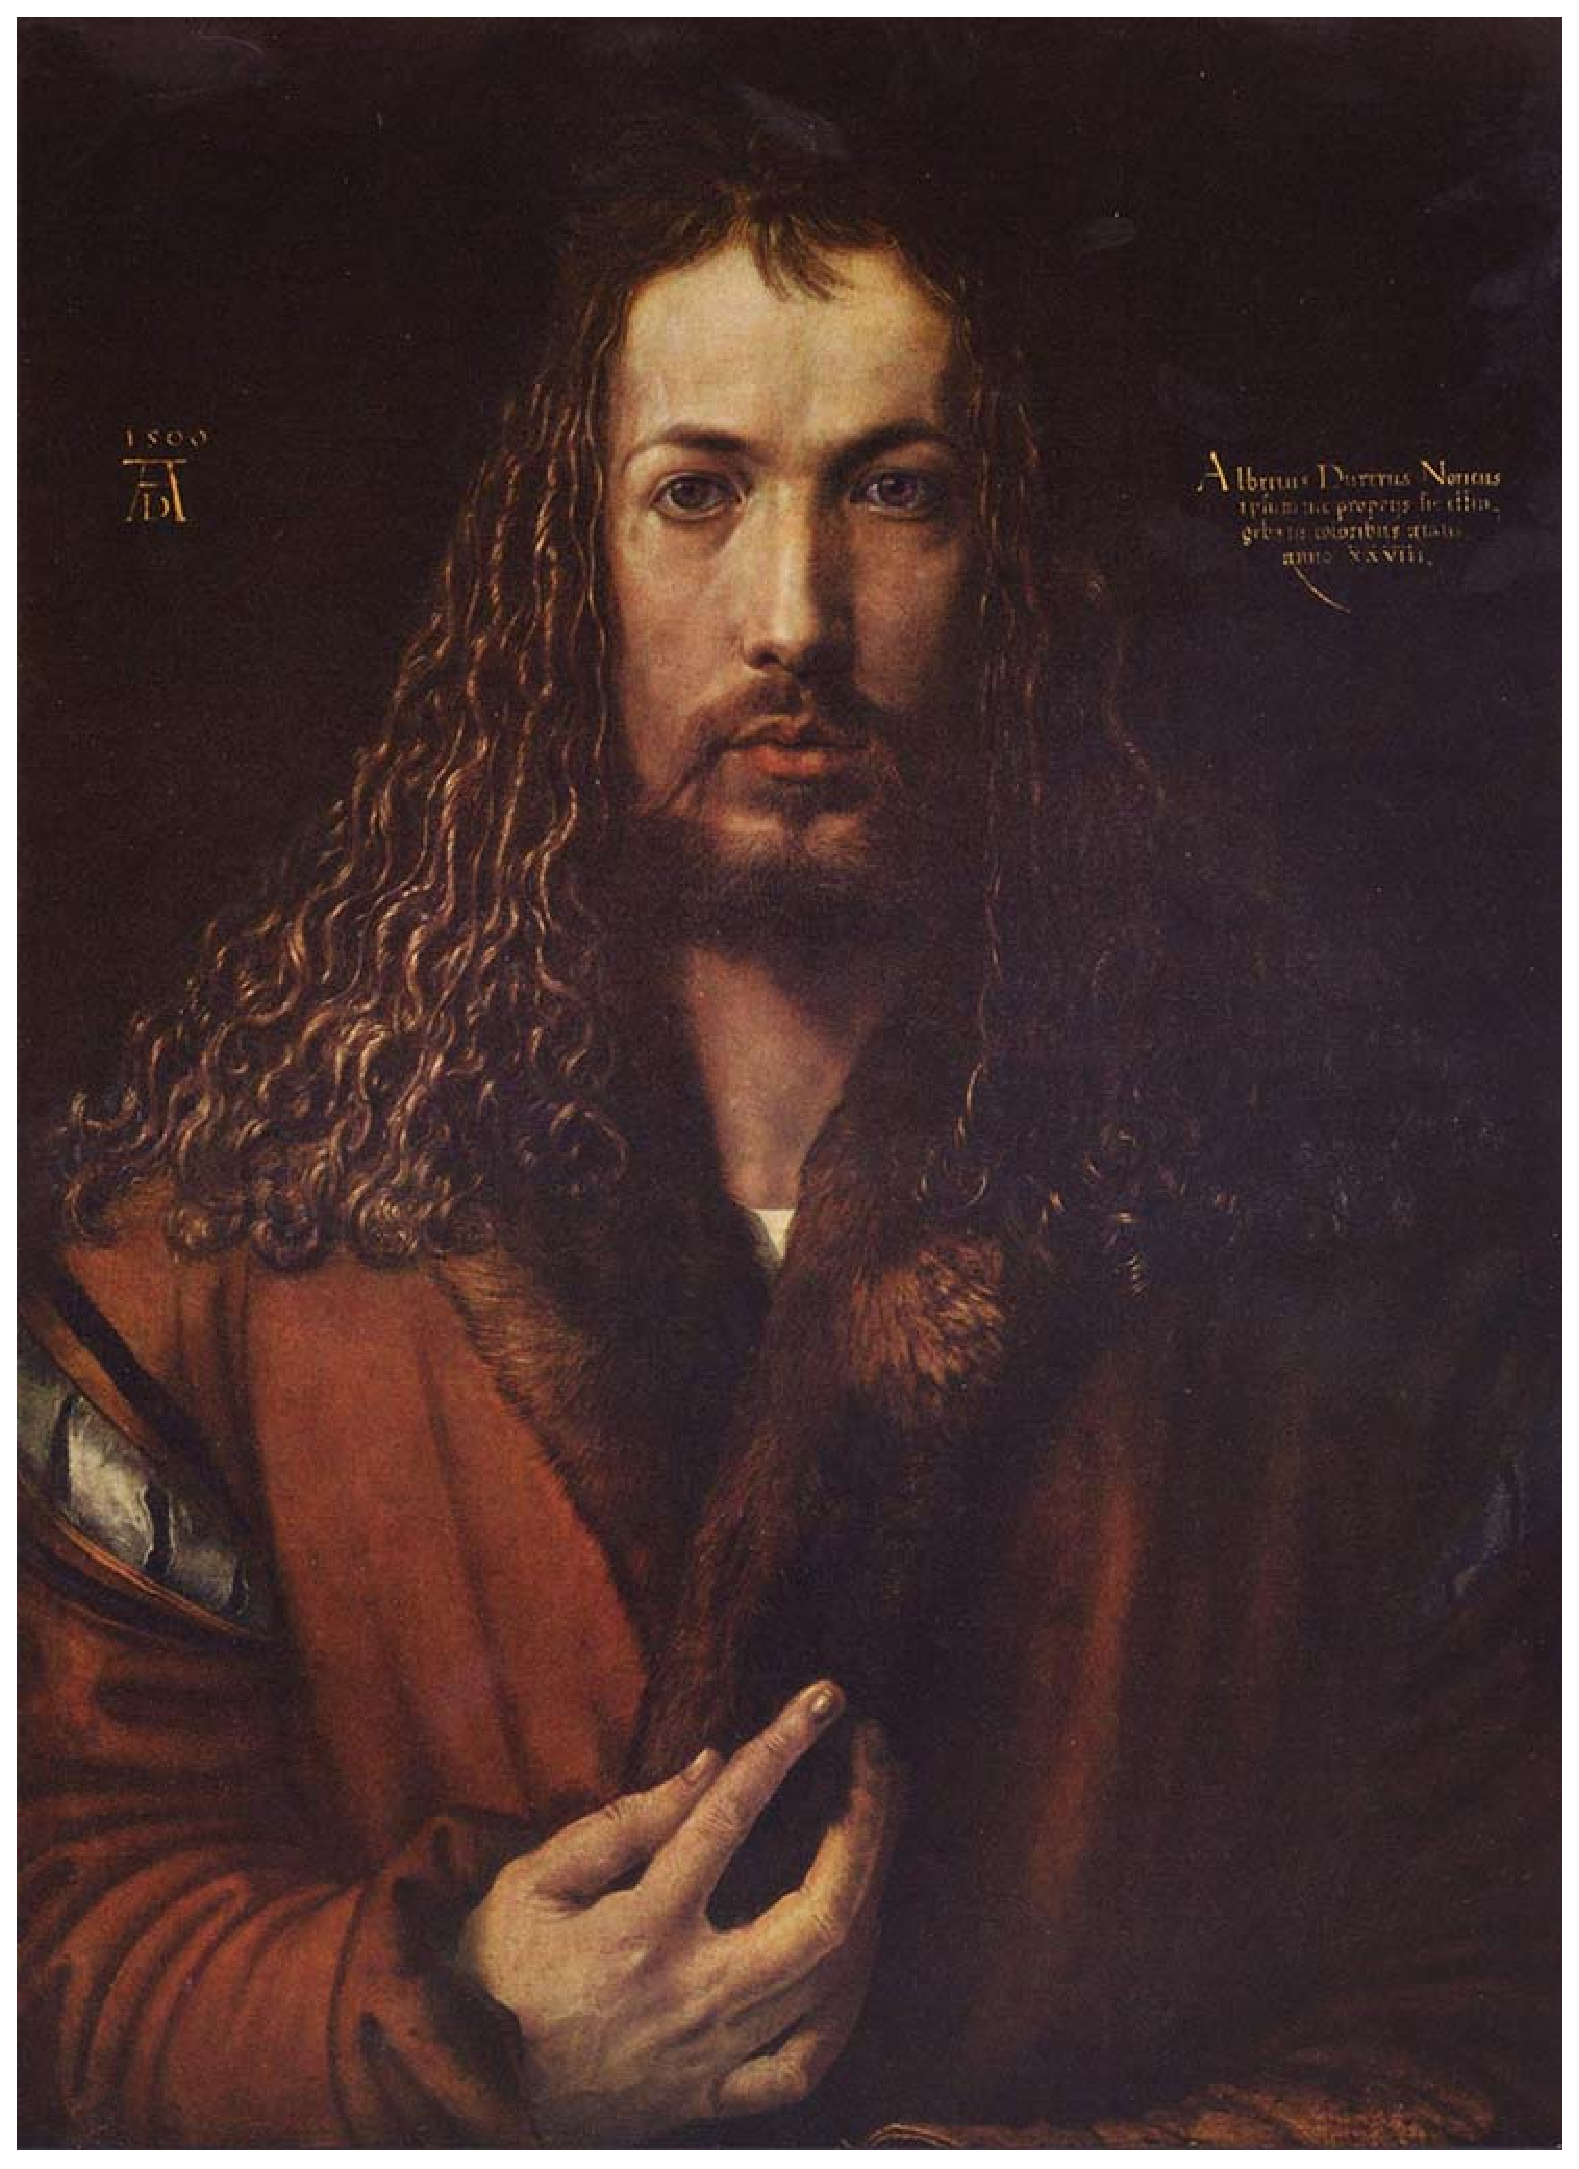
\includegraphics[scale=0.2]{Durer.eps}
\caption{Albert Durer self portrait.}
\end{figure}










G.C. Shephard \cite{Sh} posed in 1975 the problem to determine whether all convex polyhedra have a net. Experimental results do not give us enough information to expect a positive or negative answer to the problem. However, Mohammad Ghomi solved a similar problem, which is to develop any polyhedron after a suitable stretching in one direction (theorem \ref{Str} below). In particular, every polyhedron is affinely equivalent to one with a net, and having a net does not depend on the combinatorial structure of the polyhedron. 

\begin{teorema}\label{Str}
{\rm Let $P$ be a convex polyhedron, then there is a linear stretching $L$, such that $L(P)$ has a net.}
\end{teorema}



Let $\xi $ be a direction not orthogonal to any line determined by two vertices of $P$. Applying a rotation sending $\xi $ to $e_1 $, we obtain a polyhedron such that no edge is orthogonal to $e_1$. Therefore, after a suitable stretching in the direction of the $x$ axis, all the edges of the obtained polyhedron $Q$  form an angle of less than $\frac{\pi}{20 N}$ with $e_1$, where $N$ is the number of edges of $P$.


We now define an ordering on the set of vertices of $Q$. We say that $v \leq v^{\prime}$ if the first coordinate of $v$ is less or equal than the first coordinate of $v^{\prime}$. We will denote by $y$ and $z$ the minimal and maximal vertices respectively.

We define an \textit{ascending sequence} as a set of vertices $\{ p_0, p_1, \ldots , p_n   \}$ such that $p_i \leq p_{i+1}$ and $p_i p_{i+1}$ are connected by an edge for all $i \in \{ 0,1, \ldots, n-1 \} $. We say that a spanning tree $T$ with root $z$ is \textit{increasing} if for any vertex $v\in Q$ there is a (unique) ascending sequence from $v$ to $z$ contained in $T$. 

Note that all leaves of an increasing tree form an angle close to $\pi$ with $e_1$. Otherwise, the path in $T$ joining the corresponding leaf to $z$ wouldn't be an ascending sequence (see figure \ref{Mon}). Also, all the ends of the surface $Q \backslash T$ point in the direction of the $x$ axis.




\begin{figure}[h]
\centering
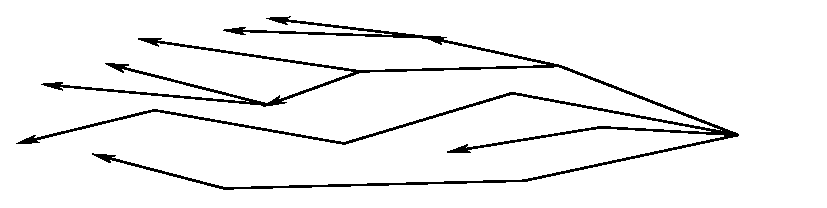
\includegraphics[scale=0.84]{Mono2.eps}
\caption{Leaves of an increasing tree point leftwards and ends of its complement point rightwards.}\label{Mon}
\end{figure}



In what follows, we give a proof of theorem \ref{Gho} below, which clearly implies theorem \ref{Str}. 



\begin{teorema}\label{Gho}
{\rm \textbf{(Ghomi)} If $Q$ is cut along any increasing tree $T$, then it can be unfolded without overlapping in $\R ^2$.}
\end{teorema}


\section*{Preliminaries}



Let $a, b, c$ be vertices such that $ab $ and $ac$ are connected by edges. We will denote by $\measuredangle bac $ the intrinsic angle at $a $ from $ab$ to $ac$ measured counterclockwise. Note that by convexity

\begin{equation}\label{Alex}
\measuredangle bac + \measuredangle  cab  < 2\pi.
\end{equation} 

For distinct $x,y,z \in \R^2$, $arg (x)$ will denote the argument from $-\pi$ to $\pi$ of $x$ as a complex number, and $\angle yxz $ will denote the angle at $x$ measured counterclockwise. We will say that two sequences of points in $\R ^2$ \textit{cross} if the broken line's determined by them do so. 
 

\begin{lema} \label{Arm}
{\rm \textbf{(Arm Lemma)} Suppose $\{ u_0, u_1, \ldots , u_m     \}, \{ v_0, v_1, \ldots , v_m      \} \subset \R^2$ satisfy
\begin{itemize}
\item $u_0 = v_0$.
\item $\vert u_j - u_{j-1} \vert = \vert v_j - v_{j-1}  \vert$ for $j=1,2, \ldots, m$.
\item $u_{j }- u_{j-1} $ and $v_j - v_{j-1} $ are almost horizontal for $j = 1, 2, \ldots , m$ (their argument is in $\left( -\frac{\pi}{10},\frac{\pi}{10} \right)$ ).
\item $arg (v_{i} - v_{i-1} )\geq arg (u_{i} - u_{i-1})$ for $i \in \{ 1, 2, \ldots, m \} $.
\end{itemize}

Then $\{ u_0, u_1, \ldots , u_m     \}$ and $ \{ v_0, v_1, \ldots , v_m      \}$ do not cross and $v_m - u_m$ is almost vertical (its argument lies in the interval $\left(  \frac{\pi}{2} - \frac{\pi}{10} , \frac{\pi}{2} + \frac{\pi}{10}  \right)$ ) 
}
\end{lema}



\begin{rem}
{\rm One can observe from figure \ref{Tet} that this lemma does not hold if  we remove the condition of $u_{j }- u_{j-1}$ and $ v_j - v_{j-1} $ being almost horizontal. Here is where we use the stretching. 
}
\end{rem}




\textbf{Proof of the lemma: }We will prove this lemma by induction on $m$. The case $m=1$ is elementary plane geometry.


Suppose it holds for $m=\nu$ and take $m = \nu +1$. Construct another sequence $\{ w_1, w_2, \ldots, w_m   \}$ such that $w_1 = v_1$ and $u_{j+1}u_jw_jw_{j+1} $ is a parallelogram for $j \in \{ 1, 2, \ldots , m-1\} $. Applying the induction hypothesis to $\{ w_1, w_2, \ldots w_m   \}$ and $\{v_1, v_2, \ldots, v_m  \}$, we see that they do not cross and $arg( w_{m} - v_m) \in \left(  \frac{4 \pi}{10} , \frac{6\pi}{10}  \right)$. Also, $arg(u_m - w_m )= arg (u_1 - w_1) = arg (u_1 - v_1) \in \left(  \frac{4 \pi}{10} , \frac{6\pi}{10}  \right)$, which implies $arg(u_m - v_m)\in \left(  \frac{4 \pi}{10} , \frac{6\pi}{10}  \right)$.

\hfill $\Box$


\begin{figure}[h]
\centering
\psfrag{A}{$u_0$}
\psfrag{B}{$u_1$}
\psfrag{C}{$u_2$}
\psfrag{D}{$u_3$}
\psfrag{E}{$u_4$}
\psfrag{F}{$v_1$}
\psfrag{G}{$v_2$}
\psfrag{H}{$v_3$}
\psfrag{I}{$v_4$}
\psfrag{J}{$w_2$}
\psfrag{K}{$w_3$}
\psfrag{L}{$w_4$}
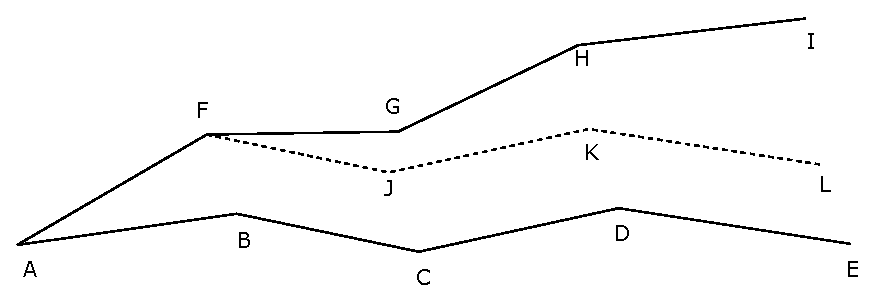
\includegraphics[scale=0.95]{arms.eps}
\caption{Proof of arm lemma.}
\end{figure}


% I am unsure how to do a bridge between arm lemma and the following lemma

\begin{lema}\label{Argument}
{\rm Let $S$ be a flat surface homeomorphic to a closed disc. Consider a map $f: S \rightarrow \mathbb{R}^2$ such that restricted to the interior of $S$ is an isometric immersion. Then $f$ is injective if and only if $f(\partial S)$ is a simple closed curve. 
}
\end{lema}


\textbf{Proof: }One implication is trivial. The other one follows from the fact that for conformal maps $f: S \rightarrow \mathbb{R}^2$, the number of preimages $f^{-1}(x)$ equals the winding number $I(f(\partial S), x )$ for all $x \in \R^2  \backslash f(\partial S)$, which is a standard fact in complex analysis (\cite{Ma}, p. 384). If $f(\partial S)$ is a simple closed curve, by Jordan Curve Theorem \cite{Ha} the winding number $I(f(\partial S), x )$ equals 0 or 1, then the function is injective.


\hfill $\Box$

\section*{Proof of Theorem \ref{Gho}}

First, construct an unfolding $f_T$ of $Q_T$ in which the images of all the edges are almost horizontal (they form an angle less than $\frac{\pi}{10}$ with $e_1 \in \R ^2$). Next, we are going to prove that $f_T(\partial Q_T)$ does not self intersect.

Consider $y^{\prime} = f_T(y) \in \R ^2$. Then, starting at $y^{\prime}$, the counterclockwise image of $\partial Q_T$ is a sequence of piecewise linear curves (broken lines) going almost horizontally rightwards and leftwards, alternately. We are going to denote the first broken line going right as $R_1$, the first one going left as $L_1$, and so on. Since $T$ is ascending, when we switch from going rightwards to leftwards, we rotate counterclockwise and when we switch from going leftwards to rightwards, we rotate clockwise (see figure \ref{Cro}). 



\begin{figure}[h]
\centering
\psfrag{A}{$1$}
\psfrag{B}{$2$}
\psfrag{C}{$3$}
\includegraphics[scale=0.7]{Bry.eps}
\caption{The image of the boundary is a sequence of broken lines going rightwards and leftwards alternately.}\label{Cro}
\end{figure}




\begin{prop}\label{Zig}
{\rm As defined above, if the sequence of broken lines $R_1L_1R_2\ldots$ 
$ L_n$ doesn't self intersect, then $R_1L_1 R_2 \ldots L_nR_{n+1}$ doesn't self intersect either.  

}
\end{prop}




\textbf{Proof: }The proof goes by induction on the number $n$ of times it has gone leftwards (in figure \ref{Cro}, $n=3$). For the case $n=1$, observe that the condition $arg (v_{i} - v_{i-1} )\geq arg (u_{i} - u_{i-1})$ for $i =1, 2, \ldots, m$ in the arm lemma is implied by $arg (v_1 - v_0 )\geq arg (u_1 - u_0)$ and $\angle v_{i+1}v_iv_{i-1}+ \angle u_{i-1}u_iu_{i+1} \leq 2\pi$ for $i\in \{ 1,2, \ldots, m-1\}$. Therefore the arm lemma completes the base of induction.

Suppose the assertion is true for $n \leq k$ and consider the case $n=k+1$.  Note that the edges of $\partial Q_T$ are paired in such a way that we glue paired edges together to obtain $Q$ from $Q_T$. Each one will be called the \textit{dual} of the other.

Observe that when we start $R_2$, we are traveling the dual edges of the leftmost part of $L_1$. If the length of $R_2$ is greater than or equal to the length of $L_1$, we can apply the induction hypothesis to $R_2L_2R_3 \ldots L_nR_{n+1}$ and the result will follow. 

If the length of $R_2$ is less than the length of $L_1$, we extend $R_2 $ with a broken line $S$ parallel to $L_1$ minus the dual of $R_2$. By the arm lemma, $S$ will be above $L_1$ (see figure \ref{S}), and by the induction hypothesis $S$ does not touch $L_2R_3 \ldots L_nR_{n+1}$ so this finishes the proof of proposition \ref{Zig}.

\hfill $\Box$



\begin{figure}[h]
\centering
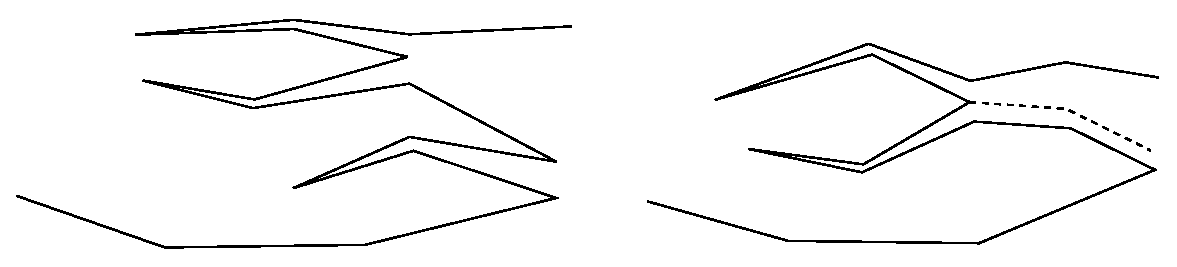
\includegraphics[scale=0.7]{S.eps}
\caption{On the left $R_2$ and $L_1$ have the same length, on the right we construct $S$ in blue.} \label{S}
\end{figure}




Now, the image of $\partial  Q_T$ will self intersect for the first time in a point $y^{\prime\prime}$ while going leftwards. Because $T$ is increasing, $f_T(\partial Q_T)$ contains a simple closed curve $\gamma$ starting at $y^{\prime \prime}$ consisting of a sequence of broken lines turning clockwise when changing from going leftwards to rightwards and counterclockwise in the other case.




\begin{figure}[h]
\centering
\psfrag{A}{$y^{\prime}$}
\psfrag{B}{$y^{\prime\prime}$}
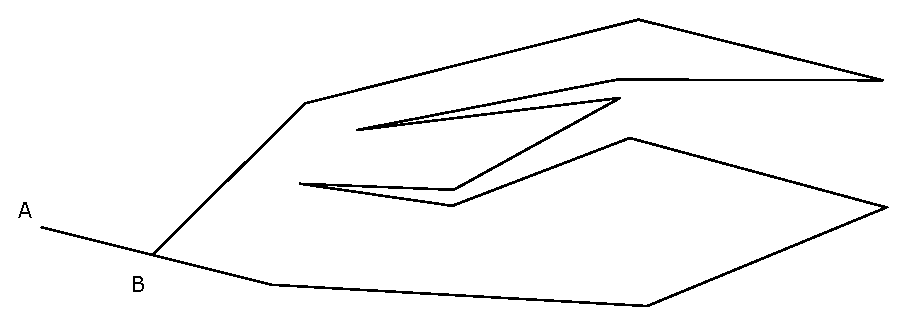
\includegraphics[scale=0.7]{Prime.eps}
\caption{The image of $\partial Q_T$ first self intersects at $y^{\prime \prime}$.}
\end{figure}


Since all ends point rightwards, we can contract the curve $\gamma$ to the point  $y^{\prime \prime}$ moving leftwards all the time. Such contraction can be performed in the same way in $Q_T$. Therefore only one point of $\partial Q _T$ is sent to $y^{\prime \prime}$. This is only possible if $y^{\prime} = y^{\prime \prime}$ and $f_T$ restricted to $\partial Q_T$ is injective.


Applying lemma \ref{Argument} with $S=Q_T$ we get that $f_T$ is a net, completing the proof.


\begin{thebibliography}{9}

\bibitem{Du} A. Durer \textit{The painter's manual.} Literary remains of Albrecht Durer. Abaris Books. 1977.

\bibitem{Gh} M. Ghomi, \textit{Affine unfoldings of convex polyhedra.} Geom. Topol., 18(5):3055-3090, 2014. 
  
  
  \bibitem{Ha}
  T. Hales, \textit{The Jordan curve theorem, formally and informally.} The American Mathematical Monthly, 114 (10): 882-894. 2007.

\bibitem{Ma}
  J. Marsden, M. Hoffman,  \textit{Basic complex analysis.} Third Edition, W.H. Freeman, NY. 1999.  
  

\bibitem{Sh} 
G. C. Shephard, \textit{Convex polytopes with convex nets.} Math. Proc. Cambridge Philos. Soc., 78(3):389-403, 1975. 
  
\end{thebibliography}
















\end{document}


